\documentclass[letterpaper]{article}
\usepackage[margin=1in]{geometry}
\usepackage{times}
\usepackage{hyperref}
\usepackage{enumitem}
\usepackage{graphicx}
\usepackage{amssymb}
\usepackage{multirow}
\usepackage{float}


\title{\textbf{Bayesian Network Modeling of NFL Game Stats and Market Signals for Value Identification}}

\author{
  Leland Weeks\\
  \texttt{lhw22@drexel.edu}
  \and
  Johnny Belichev\\
  \texttt{jb4458@drexel.edu}
  \and
  Ishant Somal\\
  \texttt{is488@drexel.edu}
}

\date{June 4, 2026}

\begin{document}

\maketitle


\section{Abstract}

This project studies whether NFL betting market signals contain predictive information beyond what is already captured by game statistics. Specifically, we evaluate whether line movement and closing market information improve prediction of against-the-spread outcomes after accounting for game fundamentals such as offensive efficiency, defensive efficiency, turnover margin, and recent team performance. We use a dataset of 3,990 NFL games across 15 seasons, combining game statistics from NFLverse with historical betting market data from Sportsbook Review. Our approach compares stats-only, market-only, and combined feature configurations using Naive Bayes as a baseline and Bayesian Network structure-learning methods, including Hill Climbing and the PC algorithm, to test conditional relationships among game fundamentals, market signals, and ATS outcome. The results show that market signals did not produce a clear predictive improvement in classification accuracy beyond game statistics. The combined configuration that included market features, however, achieved the best probability calibration (the lowest log loss) of all nine ablations, indicating that market signals improve the confidence of predictions even when they do not change which class is predicted.  The contribution of this project is not a betting system, but a conditional-dependence analysis of information overlap between NFL game statistics and betting market behavior. 

\section{Introduction}

NFL game outcomes can be studied through two major information sources: team performance statistics and betting market behavior. Game statistics describe what teams have done on the field, including efficiency, turnovers, scoring, and recent performance. Market signals, such as opening spreads, closing spreads, moneylines, totals, and line movement, reflect how sportsbooks and bettors price a game before kickoff. Both sources may contain useful information, but it is not obvious whether they contain independent information. 

The central question of this project is whether line movement contains predictive value beyond game statistics. In other words, after accounting for game fundamentals, does market movement still help predict whether a team covers the spread? This question is connected to market efficiency. Sports betting markets are often treated as relatively efficient because closing lines summarize large amounts of available information. However, market efficiency does not mean markets are always perfect. Small inefficiencies may still exist. We frame this as both a prediction problem and a conditional-dependence problem. Rather than only asking which model performs best, we also examine whether the learned Bayesian Network structures support a direct relationship between line movement and ATS outcome.  

The contributions of this work are threefold (1) the first formal test of conditional independence between NFL game statistics, betting market signals, and ATS outcome using Bayesian Network structure learning, (2) a calibration-versus-accuracy analysis of whether market information adds value beyond game statistics, and (3) a dual-algorithm structure-learning design in which the constraint-based PC algorithm independently validates the score-based Hill Climbing result. 


\section{Related Work}

This project builds on three areas of prior work: Bayesian Networks for sports prediction, models that combine statistics with betting odds, and studies of sports betting market efficiency. 

Constantinou, Fenton, and Neil developed Bayesian Network models for association football prediction, showing that BNs can represent uncertain relationships between team strength, form, and match outcomes [3], [4]. Their work demonstrates that probabilistic graphical models are useful in sports forecasting. However, their models focus mainly on game-related factors and do not treat betting market movement as a separate source of information. 

Other research combines historical performance data with bookmaker odds. Egidi, Pauli, and Torelli use a hierarchical Bayesian model that blends team history with betting odds [5]. Hubáček, Šourek, and Železný study machine-learning methods that compare model predictions against bookmaker odds to identify potential betting opportunities [6]. These studies show that market information can be useful, but they generally treat odds as predictive features rather than testing whether market movement adds information after conditioning on game statistics. 

A third group of studies focuses directly on betting market efficiency. Simon analyzes real-time betting line movement and finds that betting markets are often reliable but not always fully efficient [7]. Moskowitz studies sports betting through the lens of asset pricing and market behavior [8]. Szalkowski and Nelson examine NFL opening and closing lines as predictors of game outcomes [9]. These works are closely related to our topic, but they do not combine game statistics and market movement inside a Bayesian Network framework. 

Our project differs by combining these perspectives. We use Bayesian Network methods to test whether NFL market movement has a direct relationship with ATS outcome after accounting for game fundamentals. The goal is not simply to build a betting model, but to study information overlap between game statistics and market signals. 

\section{Approach}

We construct a combined dataset using two sources. Game statistics come from nflverse, while market information comes from Sportsbook Review historical odds data. The datasets are joined by season and matchup using home and away teams. The final dataset contains 3,990 NFL games over 15 seasons, with both football performance variables and betting market variables. 

The prediction target is against-the-spread outcome, represented as a three-class classification problem: cover, loss, or push. A cover means the selected side beats the spread, a loss means it fails to beat the spread, and a push means the final margin equals the spread. Pushes are rare, which creates a class-imbalance issue addressed in the evaluation section. 

Our features are divided into two groups. Game-stat features include offensive efficiency, defensive efficiency, turnover margin, and rolling team performance. Market features include opening spread, closing spread, line movement, moneyline information, and totals. To prevent data leakage, rolling features are calculated only from games that occurred before the current game. The current game’s ATS result is never used as an input feature. 

Because the Bayesian Network structure-learning algorithms require categorical inputs, all continuous features were discretized into three ordinal bins before being passed to the Hill Climbing and PC models. For example, the closing spread was binned by magnitude into small, medium, and large bins. Naive Bayes, by contrast, used the continuous feature values directly through Gaussian likelihoods, which is the primary reason its accuracy exceeds that of the network models. The data were partitioned into training and test sets with an 80/20 split ratio, and structure learning and inference were implemented using the pgmpy python library. 

We evaluate three feature configurations. The stats-only configuration uses only game fundamentals. The market-only configuration uses only betting market variables. The combined configuration uses both groups together. This ablation design directly tests whether market signals add predictive value beyond statistics alone. 

Naive Bayes serves as the baseline model. Although its independence assumption is unrealistic for football data, it provides a useful comparison point. Since many features are continuous, we use Gaussian Naive Bayes. The main Bayesian Network model uses structure learning to identify dependencies among variables. Hill Climbing is used as the primary score-based structure-learning method, while the PC algorithm is used as a constraint-based validation check. 

Models are evaluated using two metrics (1) classification accuracy, which measures hard-prediction performance, and log loss, which measures probability calibration.  

\begin{figure}[H]
	\makebox[\textwidth][c]{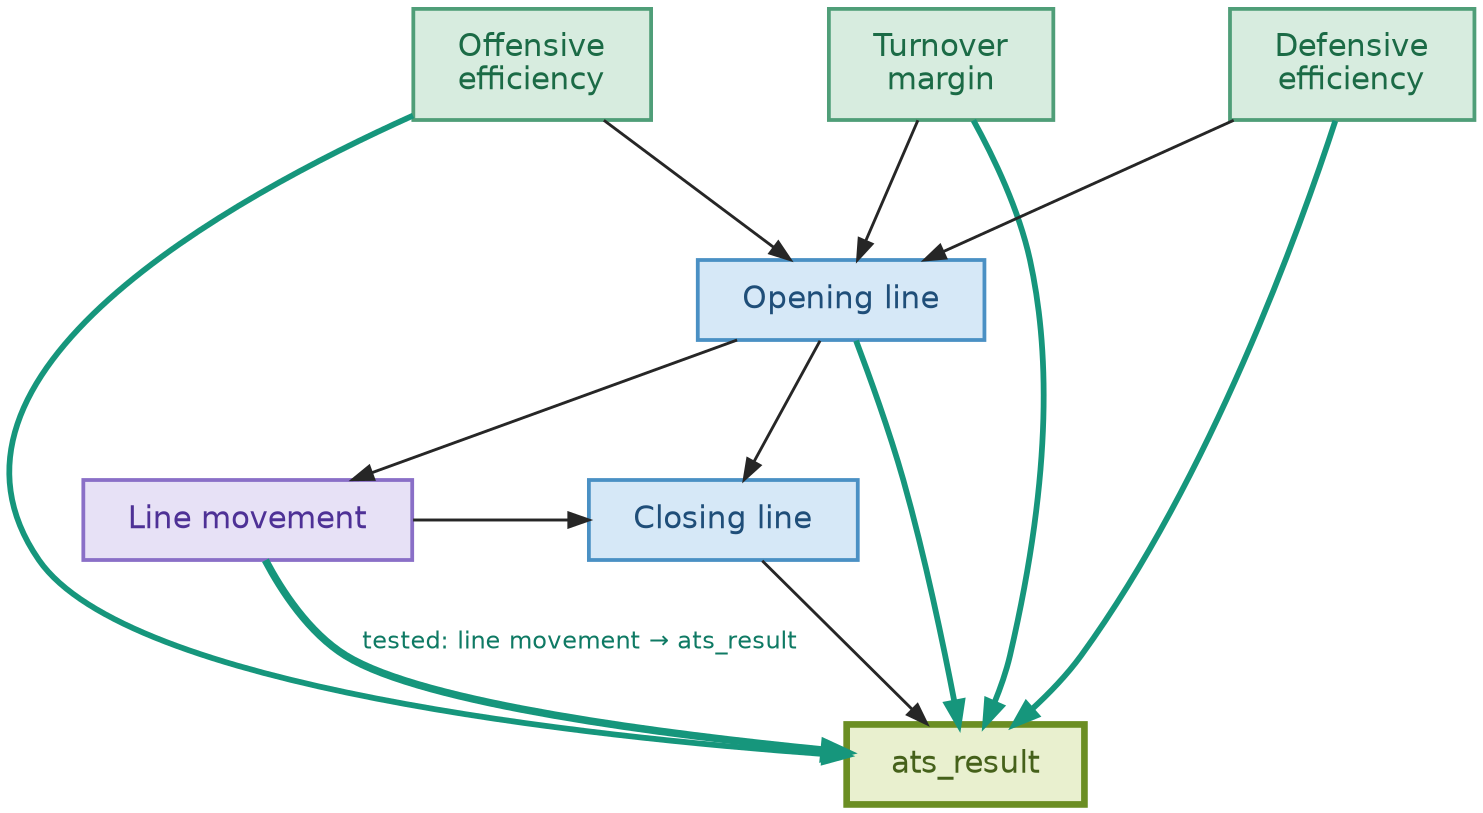
\includegraphics[width=0.50\linewidth]{assumed_domain_dag.png}}
	\caption{Assumed domain DAG used to seed structure learning.}
	\label{fig:assumed-dag}
\end{figure}

The expected domain structure is that game fundamentals influence the opening line, market activity produces line movement, and the closing line represents the final market consensus. The key question is whether line movement also connects directly to ATS outcome.  

\section{Results / Evaluation}

Before the table can be interpreted, the majority-class baseline requires explanation. In a three-class problem where one class represents 58.0\% of games, a model that predicts loss for every game achieves 58.0\% accuracy without learning anything. Any model that fails to exceed this threshold has no predictive value. The stats-only Naïve Bayes configuration achieves the highest accuracy of any model tested (84.1\%), using no market features. 

\begin{table}[h]
	\centering
	\begin{tabular}{|l|c|c|c|c|c|c|}
		\hline
		\textbf{Config} & \textbf{NB Acc} & \textbf{HC Acc} & \textbf{PC Acc} & \textbf{NB Loss} & \textbf{HC Loss} & \textbf{PC Loss} \\
		\hline
		Stats Only   & 84.1\% & 50.4\% & 50.4\% & 0.439 & 0.375 & 0.368 \\
		Market Only  & 56.4\% & 58.6\% & 58.6\% & 0.840 & 0.776 & 0.760 \\
		Combined     & 81.0\% & 50.4\% & 47.3\% & 0.538 & 0.375 & 0.345 \\
		\hline
	\end{tabular}
	\caption{Accuracy and log loss across all nine combinations.}
	\label{tab:ablation}
\end{table}

Table 2 reports precision, recall, and F1 for each model under the combined feature configuration. Neither Bayesian Network model predicts push in any configuration – at 3.0\% of the data, the class is too rare for the conditional probability tables to accumulate enough evidence to rank it above loss. Naive Bayes, operating on continuous Gaussian likelihoods rather than counted state combinations, is the only model to detect the class, achieving 22\% F1 on push. 

\begin{table}[h]
	\centering
	\begin{tabular}{|l|l|c|c|c|c|}
		\hline
		\textbf{Model} & \textbf{Class} & \textbf{Precision} & \textbf{Recall} & \textbf{F1} & \textbf{Support} \\
		\hline
		\multirow{3}{*}{Na\"{i}ve Bayes} & Cover & 0.81 & 0.80 & 0.81 & 259 \\
		& Loss  & 0.88 & 0.85 & 0.87 & 404 \\
		& Push  & 0.18 & 0.30 & 0.22 & 27  \\
		\hline
		\multirow{3}{*}{Hill Climbing} & Cover & 0.37 & 0.39 & 0.38 & 259 \\
		& Loss  & 0.59 & 0.61 & 0.60 & 404 \\
		& Push  & 0.00 & 0.00 & 0.00 & 27  \\
		\hline
		\multirow{3}{*}{PC Algorithm} & Cover & 0.35 & 0.44 & 0.39 & 259 \\
		& Loss  & 0.58 & 0.53 & 0.55 & 404 \\
		& Push  & 0.00 & 0.00 & 0.00 & 27  \\
		\hline
	\end{tabular}
	\caption{Model-Class results under the combined feature configuration.}
	\label{tab:per-class}
\end{table}

We ran Hill Climbing and the PC algorithm in tandem so each could check the other. Hill Climbing produced the edge ats\_result → epa\_diff as a game outcome causing the statistics that describe it, which is causally impossible. We corrected the direction using domain knowledge, and the PC algorithm independently recovered epa\_diff → ats\_result with no intervention, validating the correction. The pipeline catching and fixing a causally impossible edge is the methodology working as intended. 

\begin{figure}[h]
	\centering
	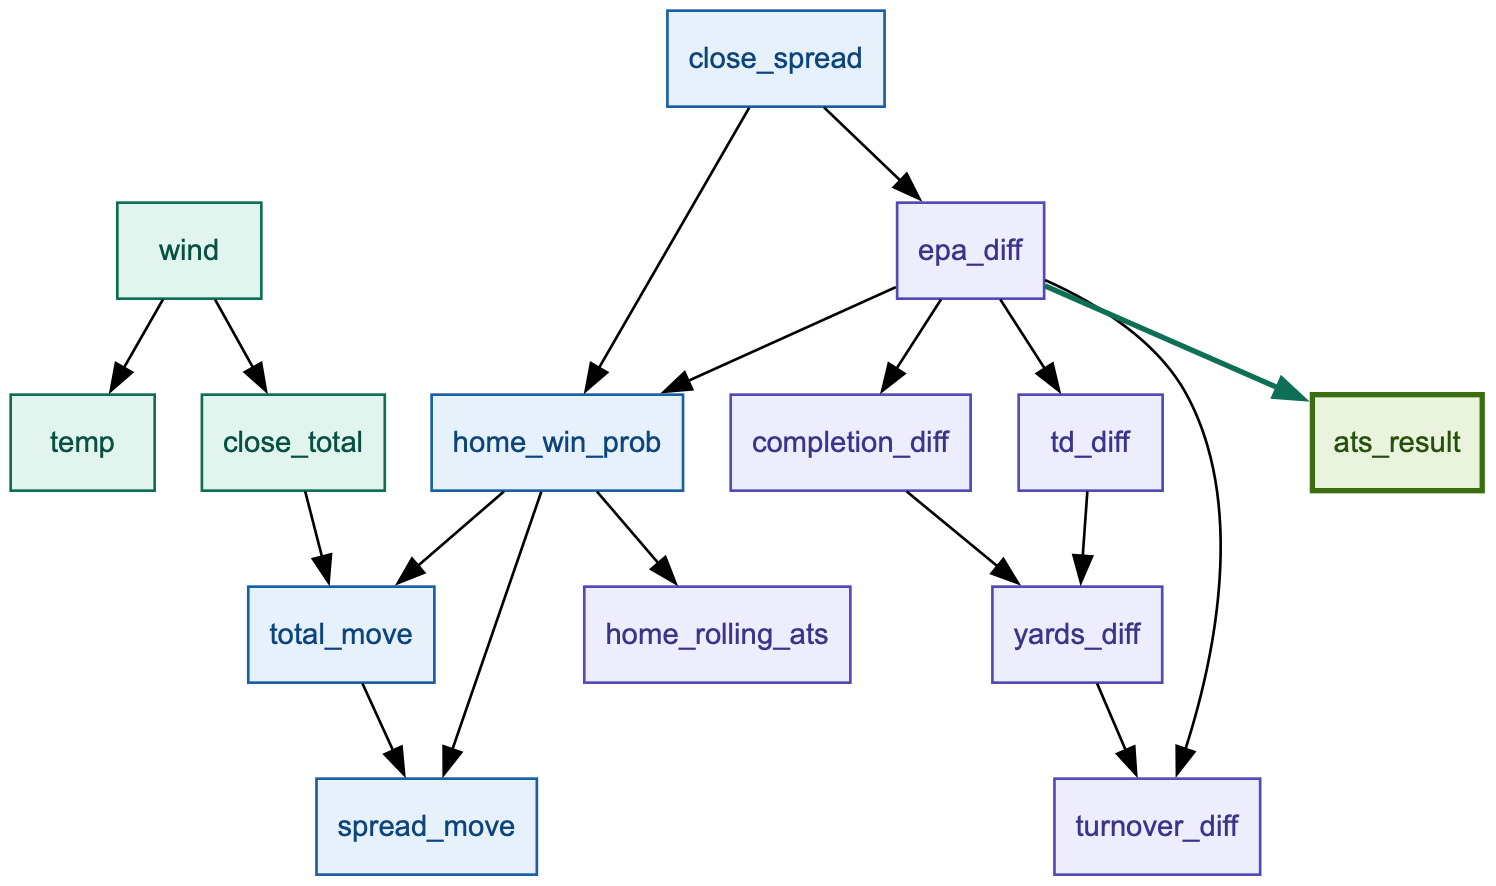
\includegraphics[width=0.50\linewidth]{hc_dag.png}
	\caption{Hill Climbing learned DAG. Green arrow indicates predictor of ats\_result.}
	\label{fig:hc-dag}
\end{figure}


The PC DAG, which gives ats\_result three direct parents – epa\_diff, home\_win\_prob, and td\_diff – the two strongest game-level margin predictors plus the market's expectation. The algorithms agree on epa\_diff → ats\_result but differ elsewhere. As expected, score-based and constraint-based learning identify the same Markov equivalence class but can orient edges within it differently. 

\begin{figure}[H]
	\centering
	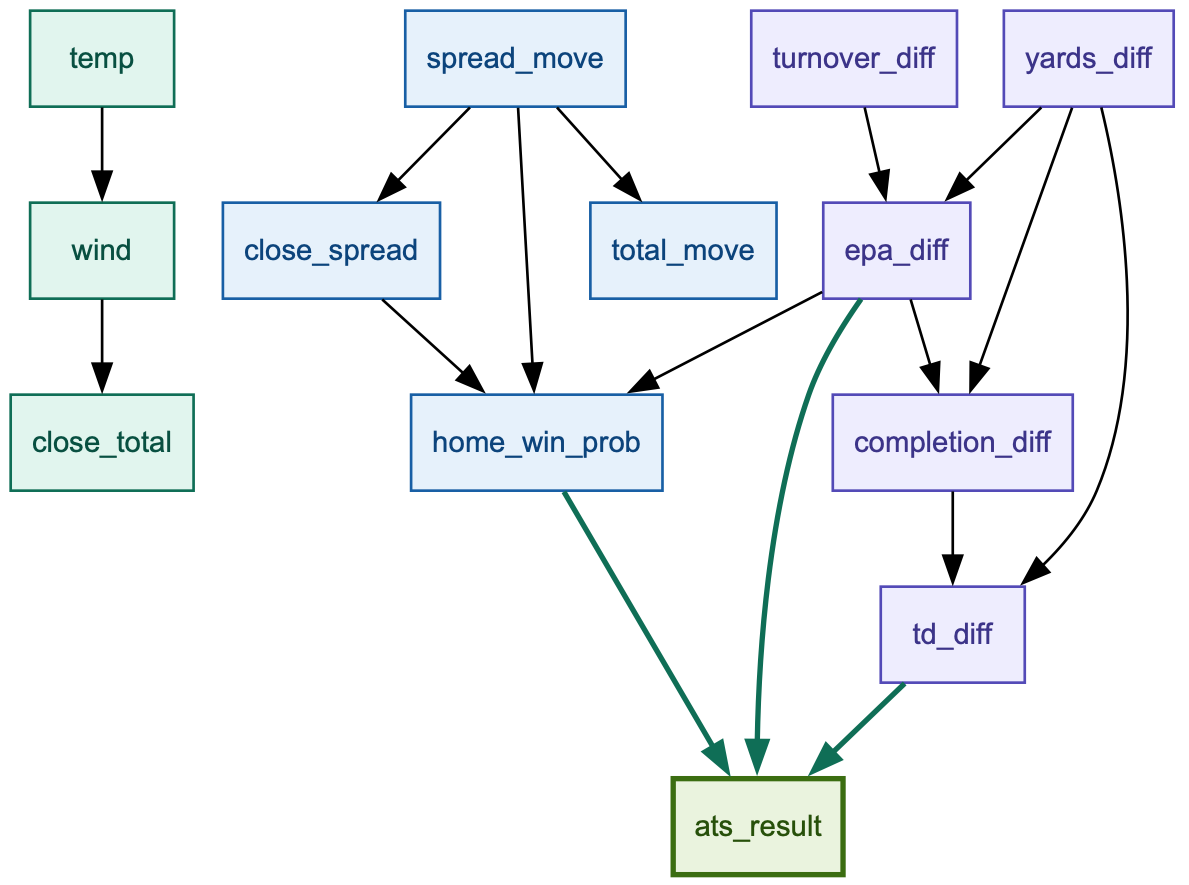
\includegraphics[width=0.50\linewidth]{pc_dag.png}
	\caption{PC Algorithm learned DAG. Green arrows indicate predictors of ats\_result.}
	\label{fig:pc-dag}
\end{figure}

Two framing points precede the findings. The game statistics are post-game measurements that correlate with ATS outcomes by construction, so the stats-only accuracy reflects information content rather than pre-game predictive power; the stats-versus-market comparison is therefore a study of information overlap, not a forecast. The central result is a divergence between accuracy and log loss: the combined PC model has the worst accuracy of all nine runs (47.3\%, below baseline), yet the best log loss (0.345). Market signals improve the probability mass assigned across all three classes without changing which class is predicted – they improve how certain the model is, not what it predicts. This is the answer to the research question. 

Two secondary findings follow. Adding market features to Naive Bayes lowers accuracy (84.1\% stats-only to 81.0\% combined) because the closing line is built partly from the same performance signals as EPA and turnover differential, and correlated features violate the model’s independence assumption. Naive Bayes also outperforms both Bayesian Networks on accuracy in every configuration because it uses continuous values, whereas the networks require binning that discards magnitude, a limitation of discretization rather than of the Bayesian Network formalism. 

\section{Conclusions}

Does line movement contain predictive information about NFL ATS outcomes beyond what game statistics encode? Adding market signals never beats game statistics alone. The stats-only Naive Bayes model is our strongest classifier and uses no market features, and the market-only networks barely clear the majority baseline. The combined PC model achieves the best log loss of all nine configurations, so the closing spread and home win probability carry uncertainty information (confidence in the prediction) the statistics do not fully encode. This is partial efficiency: the market’s hard prediction is already encoded in game statistics, but its uncertainty estimate adds information beyond them. The closing spread is not merely a point estimate; it encodes calibrated uncertainty about the outcome. 

Several limitations constrain our findings. First and most consequential, discretization – binning continuous features into three categories for the network models discards magnitude information and is the main reason the Bayesian Networks trail Naive Bayes, a continuous (Gaussian) Bayesian Network is the natural fix. (1) Neither network learns the push class – at 3.0\% of the data, the conditional probabilities never rank pushes above wins or losses. Oversampling or BDeu priors may help to address this issue. (2) Spread direction is a limitation we identified late through domain feedback: Binning the closing spread by magnitude discards directional information – a home team laying seven and one receiving seven fall in the same bin, which the model cannot recover. (3) The dataset straddles the 2018 PASPA repeal, pooling two structurally different markets. Quarterback injuries are absent for data-availability reasons and likely cap achievable accuracy; and the rolling ATS feature weights all fifteen seasons equally, which a recency-weighted version would address. 

\section{Future Work}

Future work should pursue continuous Bayesian Network variations and experiments to remove the discretization penalty, restrict analysis to the post-2018 legal-betting era to control for the PASPA repeal, recover signed spread direction to preserve key numbers, and incorporate quarterback availability data as a high-signal feature absent from the current dataset.

\begin{thebibliography}{9}

\bibitem{nflverse}
nflverse. 
\textit{nflverse: NFL data and R/Python packages for football analytics. https://nflverse.nflverse.com}.

\bibitem{sbr}
SportsBookReviewsOnline. 
\textit{NFL Odds Archives / Scores and Odds Archives. https://sportsbookreviewsonline.com/scoresoddsarchives/nfl/nfloddsarchives.htm}.

\bibitem{constantinou2012}
A. C. Constantinou, N. E. Fenton, and M. Neil, 
``pi-football: A Bayesian network model for forecasting Association Football match outcomes,'' 
\textit{Knowledge-Based Systems}, vol. 36, 2012. 
doi: 10.1016/j.knosys.2012.07.008.

\bibitem{constantinou2013}
A. C. Constantinou, N. E. Fenton, and M. Neil, 
``Profiting from an inefficient Association Football gambling market: Prediction, risk and uncertainty using Bayesian networks,'' 
\textit{Knowledge-Based Systems}, vol. 50, 2013. 
doi: 10.1016/j.knosys.2013.05.008.

\bibitem{egidi2018}
L. Egidi, F. Pauli, and N. Torelli, 
``Combining historical data and bookmakers' odds in modelling football scores,'' 
\textit{Statistical Modelling}, vol. 18, no. 5--6, 2018. 
doi: 10.1177/1471082X18798414.

\bibitem{hubacek2019}
O. Hubáček, G. Šourek, and F. Železný, 
``Exploiting sports-betting market using machine learning,'' 
\textit{International Journal of Forecasting}, vol. 35, no. 2, 2019. 
doi: 10.1016/j.ijforecast.2019.01.001.

\bibitem{simon2024}
J. Simon, 
``Inefficient forecasts at the sportsbook: An analysis of real-time betting line movement,'' 
\textit{Management Science}, vol. 70, no. 12, 2024. 
doi: 10.1287/mnsc.2022.00456.

\bibitem{moskowitz2021}
T. J. Moskowitz, 
``Asset Pricing and Sports Betting,'' 
\textit{The Journal of Finance}, vol. 76, no. 6, 2021. 
doi: 10.1111/jofi.13082.

\bibitem{szalkowski2012}
G. Szalkowski and M. L. Nelson, 
``The Performance of Betting Lines for Predicting the Outcome of NFL Games,'' 
\textit{arXiv preprint arXiv:1211.4000}, 2012.

\end{thebibliography}


\end{document}
